\subsection{Piedra, Papel o Tijeras}

\subsubsection{Descripción del juego}

Este juego es descrito en la sección \ref{section:forma-normal} y su matriz de pago se muestra en la Tabla \ref{table:pago-RPS}. El problema de programación lineal asociado es el siguiente:
\begin{equation}
\begin{array}{r r r r r r r r r r}
\max  & z &  & & & & &\\
\text{s.a.}  
&   &   & x_1  & + & x_2  & + & x_3 & =    & 1 \\
& z &   &      & + & x_2  & - & x_3 & \leq & 0 \\
& z & - & x_1  &   &      & + & x_3 & \leq & 0 \\
& z & + & x_1  & - & x_2  &   &     & \leq & 0 \\
&   &   & x_1, &   & x_2, &   & x_3 & \geq & 0
\end{array}
\end{equation}
La solución primal y dual de este problema son $(z^*, x_1^*, x_2^*, x_3^*) = (0, \frac{1}{3}, \frac{1}{3}, \frac{1}{3})$ y $(w^*, y_1^*, y_2^*, y_3^*) = (0, \frac{1}{3}, \frac{1}{3}, \frac{1}{3})$, respectivamente. Luego, el equilibrio de Nash se obtiene cuando ambos jugadores eligen cada una de las acciones con probabilidad igual a $\frac{1}{3}$.

\subsubsection{Resultados Experimentales}

En este juego, al igual que en el anterior, ambos jugadores pueden garantizar una utilidad esperada de $0$ sin importar la estrategia utilizada por su oponente, que se obtiene al elegir cada acción con igual probabilidad. Las estrategias obtenidas son presentadas en la tabla \ref{tab:estrategias-RPS}. No todas corresponden al equilibrio de Nash exacto, sin embargo, cada una de ellas es un $\varepsilon$-equilibrio de Nash con $\varepsilon < 0.006$.

\begin{table}[hbt]
    \centering
    \scriptsize
    \begin{tabular}{c|c|c|c|c}
        & E.N. & A & B & C \\ \hline
        $\sigma_1$ &  $(0.333, 0.333, 0.333)$ & $(0.332, 0.335, 0.332)$ & $(0.330, 0.334, 0.336)$ & $(0.333, 0.337, 0.330)$ \\
        $\sigma_2$ &  $(0.333, 0.333, 0.333)$ & $(0.331, 0.334, 0.335)$ & $(0.329, 0.335, 0.337)$ & $(0.336, 0.330, 0.335)$ \\ \hline
        $(v_1, v_2)$ & $(0.000, 0.000)$ & $(-0.003, -0.003)$ & $(-0.004, -0.006)$ & $(-0.004, -0.005)$ \\ \hline
    \end{tabular}
    \caption{Estrategias obtenidas del juego Piedra, Papel o Tijeras}
    \label{tab:estrategias-RPS}
\end{table}

La Tabla \ref{tab:resultados-RPS} muestra los resultados obtenidos relacionados al tiempo y número de iteraciones de los procedimientos. El procedimiento A, \textit{regret} condicional, tuvo una duración promedio de $25.715$ segundos, con un número promedio de iteraciones de $4519054.1$, obteniendo un promedio de $2.7 {\times} 10^{-6}$ segundos por iteración. Con el procedimiento B, que utiliza un vector invariante de probabilidad, se obtuvo un tiempo, número de iteraciones y tiempo por iteración promedios de $0.345$ segundos, $6601.3$ iteraciones y $5.23 {\times} 10^{-5}$ segundos por iteración, respectivamente. Por último, el procedimiento C, \textit{regret} incondicional, se obtuvo un tiempo promedio de $0.049$, el número de iteraciones promedio fue de $19321.1$, obteniendo un promedio de $2.54 {\times} 10^{-6}$ segundos por iteración.

\begin{table}[hbt]
    \scriptsize
    \centering
    \begin{tabular}{r r r | r r r | r r r}
    \multicolumn{3}{c}{A} & \multicolumn{3}{c}{B} & \multicolumn{3}{c}{C} \\ \hline
    $25.715$ & $9107389$ & $2.82 {\times} 10^{-06}$ & $0.724$ & $13750$ & $5.26 {\times} 10^{-05}$ & $0.034$ & $12967$ & $2.64 {\times} 10^{-06}$ \\
    $29.494$ & $10951479$ & $2.69 {\times} 10^{-06}$ & $0.692$ & $13257$ & $5.22 {\times} 10^{-05}$ & $0.041$ & $16096$ & $2.57 {\times} 10^{-06}$ \\
    $7.015$ & $2641656$ & $2.66 {\times} 10^{-06}$ & $0.000$ & $6$ & $4.36 {\times} 10^{-05}$ & $0.063$ & $24423$ & $2.56 {\times} 10^{-06}$ \\
    $4.610$ & $1748365$ & $2.64 {\times} 10^{-06}$ & $0.849$ & $16255$ & $5.22 {\times} 10^{-05}$ & $0.048$ & $18613$ & $2.56 {\times} 10^{-06}$ \\
    $8.051$ & $3033028$ & $2.65 {\times} 10^{-06}$ & $0.000$ & $3$ & $4.28 {\times} 10^{-05}$ & $0.082$ & $32222$ & $2.55 {\times} 10^{-06}$ \\
    $9.870$ & $3717278$ & $2.66 {\times} 10^{-06}$ & $0.000$ & $3$ & $4.28 {\times} 10^{-05}$ & $0.084$ & $33042$ & $2.54 {\times} 10^{-06}$ \\
    $2.749$ & $1037895$ & $2.65 {\times} 10^{-06}$ & $0.000$ & $3$ & $4.06 {\times} 10^{-05}$ & $0.049$ & $19316$ & $2.55 {\times} 10^{-06}$ \\
    $11.971$ & $4517546$ & $2.65 {\times} 10^{-06}$ & $0.556$ & $10644$ & $5.23 {\times} 10^{-05}$ & $0.024$ & $9601$ & $2.54 {\times} 10^{-06}$ \\
    $14.974$ & $5606070$ & $2.67 {\times} 10^{-06}$ & $0.000$ & $3$ & $3.74 {\times} 10^{-05}$ & $0.014$ & $5621$ & $2.55 {\times} 10^{-06}$ \\
    $7.532$ & $2829835$ & $2.66 {\times} 10^{-06}$ & $0.631$ & $12089$ & $5.22 {\times} 10^{-05}$ & $0.054$ & $21310$ & $2.55 {\times} 10^{-06}$ \\ \hline
    $12.198$ & $4519054.1$ & $2.70 {\times} 10^{-06}$ & $0.345$ & $6601.3$ & $5.23 {\times} 10^{-05}$ & $0.049$ & $19321.1$ & $2.54 {\times} 10^{-06}$ \\ \hline
    \end{tabular}
    \caption{Resultados del juego Piedra, Papel o Tijeras}
    \label{tab:resultados-RPS}
\end{table}

La Figura \ref{fig:regret-RPS} muestra el regret incondicional con respecto al tiempo de la última corrida para los procedimientos A, B y C. Se observa como el \textit{regret} total de ambos jugadores converge a cero.

\begin{figure}[hbt]
\caption{Gráficas del regret con respecto al número de iteraciones del juego Piedra, Papel o Tijera}
\label{fig:regret-RPS}
\centering
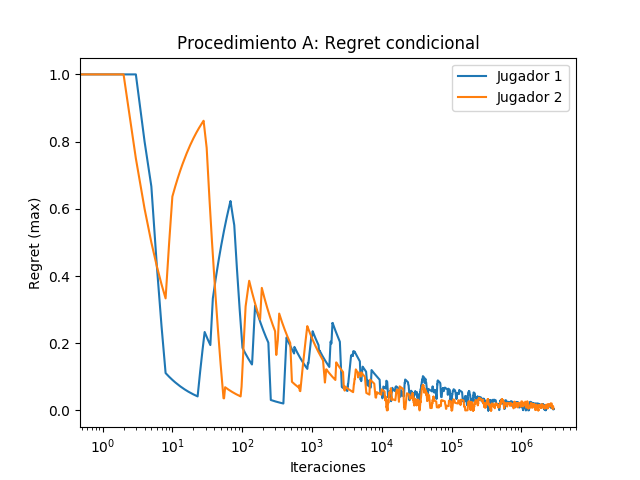
\includegraphics[width=0.45\textwidth]{graficas/RPS/procedimiento-A.png}
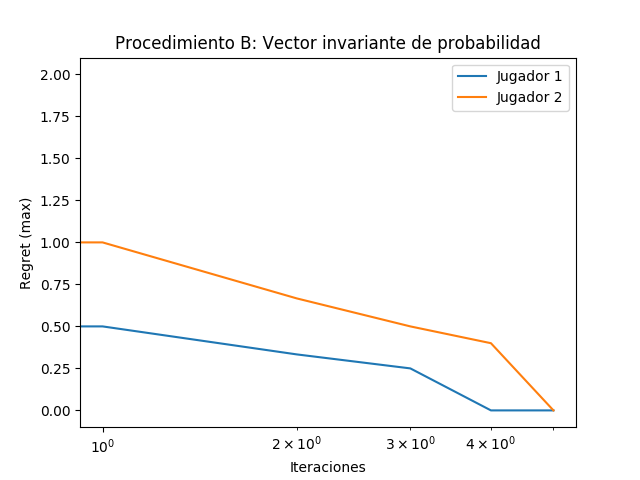
\includegraphics[width=0.45\textwidth]{graficas/RPS/procedimiento-B.png}
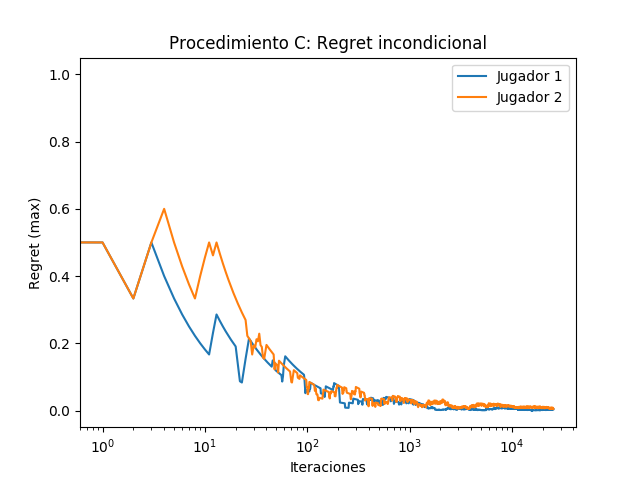
\includegraphics[width=0.45\textwidth]{graficas/RPS/procedimiento-C.png}
\end{figure}